\section{Durchführung}
\label{sec:Durchführung}
In diesem Abschnitt wird die Bestimmung der Durchlasskurve des verwendeten Bandpassfilters erläutert sowie die Messung der paramagnetischen Suszeptibilität Stoffe erklärt.

\subsection{Filterkurve des Bandpassfilters}
Es wird die Ausgangsspannung in Abhängigkeit der Eingangsfrequenz gemmessen. Es wird eine konstante Eingangsspannung an den Selektivverstärker angelegt, welcher mit einem Spannungsmessgerät verbunden ist. 
Die Eingangsfrequenz durchläuft den Bereich von $ 10 \, \unit{\kilo\hertz}$ bis $40 \, \unit{\kilo\hertz}$, dabei wird das Maximum der Ausgangsspannung $ U_{A} $ zur Eingangsspannung $ v_0$ bestimmt.


\subsection{Messung der paramagnetischen Suszeptibilität von seltenen Erden}
Es wird eine Messaperatur nach \autoref{fig:abb5} aufgebaut.
\begin{figure}[H]
    \centering
    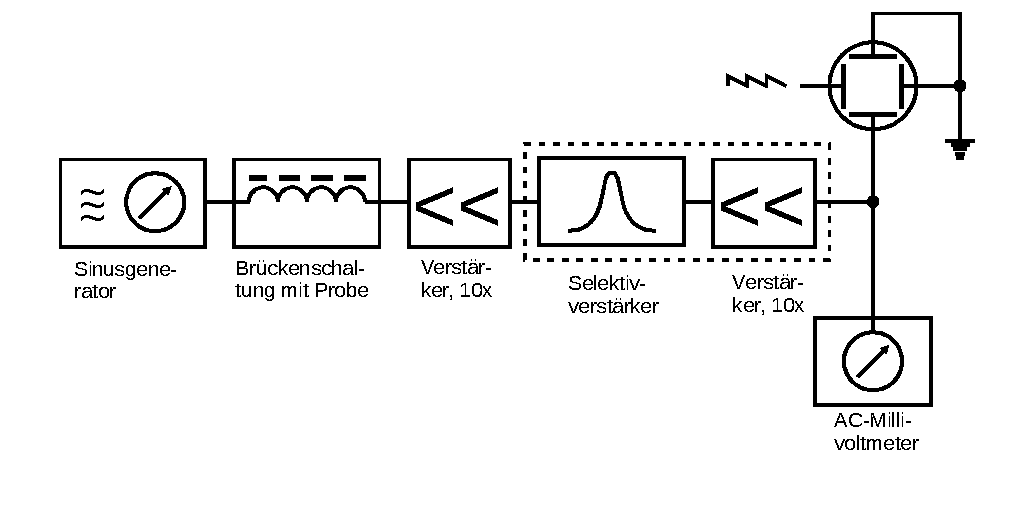
\includegraphics{figures/Abb_5.pdf}
    \caption{Blockschaltung der Messaperatur}
    \label{fig:abb5}
\end{figure} 

Die Eingangsspannung wird durch einen Frequenzgenerator erzeugt.
Die Verstärker vor und hinter dem Selektivverstärker aus \autoref{fig:abb5} werden nicht verwendet. Die Brückenspannung wird allerdings am Selektivverstärker 10-fach verstärkt. Der Selektivverstärker ist mit einem Spannungsmessgerät verbunden, das über diesen die Brückenspannung $ U_{Br}$ misst.